\documentclass[IntroMain.tex]{subfiles} 
\begin{document}
\frame{
	\frametitle{The Binomial Probability Distribution}
	\begin{itemize}
		\item The number of independent trials is denoted $n$.
		\item The probability of a `success' is $p$
		\item The expected number of `successes' from $n$ trials is $E(X) = np$
	\end{itemize}
}	
%--------------------------------------------------------------------------------------%
\frame{
\frametitle{Binomial Experiment}
A binomial experiment (also known as a Bernoulli trial) is a statistical experiment that has the following properties:
\begin{itemize}
\item The experiment consists of $n$ repeated trials.
\item Each trial can result in just two possible outcomes. We call one of these outcomes a \textbf{\emph{success}} and the other, a \textbf{\emph{failure}}.
\item The probability of success, denoted by $p$, is the same on every trial.
\item The trials are independent; that is, the outcome on one trial does not affect the outcome on other trials.
\end{itemize}
}
%--------------------------------------------------------------------------------------%
\frame{
\frametitle{Binomial Experiment}
Consider the following statistical experiment. You flip a coin five times and count the number of times the coin lands on heads. This is a binomial experiment because:
\begin{itemize}
\item The experiment consists of repeated trials. We flip a coin five times.
\item Each trial can result in just two possible outcomes : heads or tails.
\item The probability of success is constant : 0.5 on every trial.
\item The trials are independent; that is, getting heads on one trial does not affect whether we get heads on other trials.
\end{itemize}
}
%--------------------------------------------------------------------------------------%
\frame{
\frametitle{Binomial Probability}
\begin{itemize}
\item A binomial experiment with n trials and
probability $p$ of success will be denoted by
\[B(n, p)\]
\item Frequently, we are interested in the \textbf{\emph{number of successes}} in a binomial experiment, not in the order in which they occur.
\item Furthermore, we are interested in the probability of that number of successes.
\end{itemize}

}
%--------------------------------------------------------------------------------------%
\frame{
\frametitle{Binomial Probability}
The probability of exactly k successes in a binomial experiment B(n, p) is given by
\[ P(X=k) = P(k \mbox{ successes }) = \;^nC_k  \times p^{k} \times (1-p)^{n-k}\]

\begin{itemize}
\item X: Discrete random variable for the number of successes (variable name)
\item $k$ : Number of successes (numeric value)
\begin{itemize}
\item  $P(X=k)$ ``probability that the number of success is $k$".
\end{itemize}
\item $n$ : number of independent trials
\item $p$ : probability of a success in any of the $n$ trial.
\item $1-p$ : probability of a failure in any of the $n$ trial.
\end{itemize}

}


%--------------------------------------------------------------------------------------%
\frame{
\frametitle{Binomial Example }

Suppose a die is tossed 5 times. What is the probability of getting exactly 2 fours?

\textbf{Solution:}

This is a binomial experiment in which \begin{itemize}\item a success is defined as an outcome of `4'. \item the number of trials is equal to $n=5$, \item the number of successes is equal to $k=2$,\item the number of failures is equal to 3, \item  the probability of success on a single trial is 1/6, \item  the probability of failure on a single trial is 5/6.\end{itemize}
}
%--------------------------------------------------------------------------------------%
\begin{frame}[fragile]
\frametitle{Binomial Example }

Therefore, the probability of getting exactly 2 fours is:

\[P(X=2) = ^5C_2 \times (1/6)^2 \times (5/6)^3 = 0.161\]

Remark: $^5C_2 = 10$\\
\bigskip


\end{frame}

%--------------------------------------------------------%

\frame{
\frametitle{Binomial Example}

\begin{center}
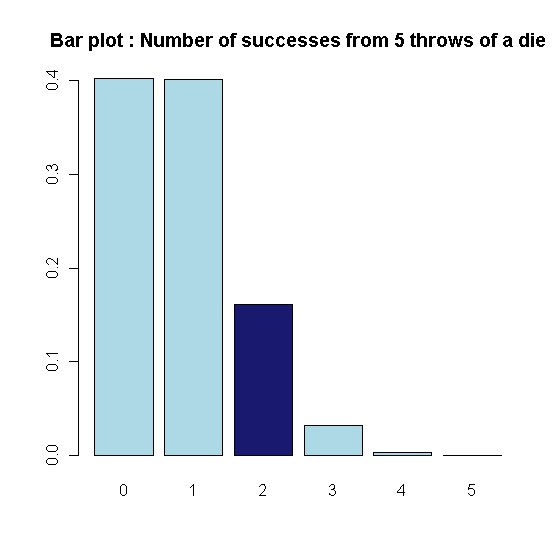
\includegraphics[scale=0.40]{images/3Bbarplot4}
\end{center}
}
%--------------------------------------------------------------------------------------%
\frame{
\frametitle{Binomial Probability}

\textbf{Remark} : The sum of the probabilities of each of the possible outcomes (i.e. no fours, one four etc) is equal to one.
\[P(X=0) + P(X = 1) + \ldots + P(X=5) = 1 \]

}
%--------------------------------------------------------%

\frame{
\frametitle{Binomial Example: At least two successes}
\begin{figure}
\centering
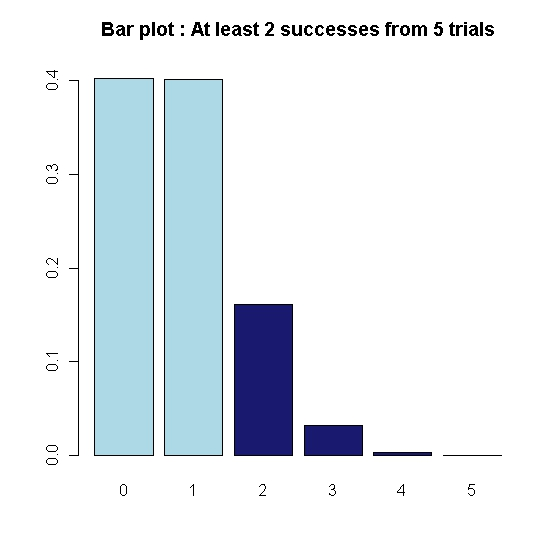
\includegraphics[width=0.7\linewidth]{images/3Bbarplot5}
\caption{}
\label{fig:3Bbarplot5}
\end{figure}

}

%--------------------------------------------------------%

\frame{
\frametitle{Binomial Example: At least two successes}
\begin{itemize}
\item Suppose we were asked to find the probability of \textbf{\emph{at least}} 2 fours.
\item Can you suggest the most efficient way of computing this?
\item Suggestion: Compute $P(X=0)$ and $P(X = 1)$.
\item Together these probabilities are the complement probability of what we require.
\item $P(X \geq 2) = 1 - ( P(X=0) + P(X = 1))$.
\item (We will continue with this in future classes).
\end{itemize}
}
%--------------------------------------------------------------------------------------%
\frame{
\frametitle{Cumulative Distribution Function}


The cumulative distribution function (c.d.f.) of a discrete random variable $X$ is the function $F(t)$ which tells you the probability that X is less than or equal to t. \\ So if X has p.d.f. P(X = x), we have:

\[ F(t) = P(X \leq t) = \sum_{(i=0)}^{(i=t)} P(X = x) \]

In other words, for each value that X can be which is less than or equal to $t$, work out the probability that X is that value and add up all such results.

}




%--------------------------------------------------------%

\begin{frame}[fragile]
\frametitle{Binomial Example: Sample Problem}

Suppose there are twelve multiple choice questions in an English class quiz. Each question has five possible answers, and only one of them is correct. Find the probability of having four or less correct answers if a student attempts to answer every question at random.
\end{frame}

%--------------------------------------------------------%

\begin{frame}[fragile]
	\frametitle{Binomial Example: Sample Problem}

\textbf{Solution:}
Since only one out of five possible answers is correct, the probability of answering a question correctly by random is $1/5=0.2$. We can find the probability of having exactly 4 correct answers by random attempts as follows.(Blackboard. Correct Answer is 13.29\%)
%\begin{verbatim}
%> dbinom(4, size=12, prob=0.2)
%[1] 0.1329
%\end{verbatim}
\end{frame}
%--------------------------------------------------------%




\end{document}







